\input{chapter-header.tex}
% ===========================================================================
\chapter{Achieving Software Evolution with Object Spaces}
\minitoc
% ===========================================================================
\introduction
% ===========================================================================

We will present three techniques for software evolution, and how their challenges are overcame with our object spaces model: bootstrapping, tailoring, runtime monitoring and modification.

% ===========================================================================
\section{Bootstrapping}
% ===========================================================================

The concept of \emph{bootstrap} is  well known in the context of compilers. For example, a bootstrapped C compiler is a compiler that, by using its own source code, can produce another compiler with its same behavior. We can generalize the process to obtain a bootstrapped system as the following.

\begin{definition}[Bootstrap Process]
A bootstrap is a process that defines a system S using S itself, by providing a self-describing specification of its own structure and behavior.
Alternatively, we can say a bootstrap is a process that defines a system S using a specification that can be fully processed by S itself.
\end{definition}

Once bootstrapped, a system relies only on itself and its specification to re-generate its own infrastructure.
Improvements such as bugfixing, speed optimizations and mutations of the language are performed by modifying the specification and recreating the system. 
We can thus define a bootstrapped system as the following. 

\begin{definition}[Bootstrapped System]
A bootstrapped system is a system that supports its own evolution.
\end{definition}

\subsection{Evolution by Bootstrapping}

When the system in construction is introduced into its own recreation process, this process is named a \emph{bootstrap}. The most prominent example is the C compiler which was initially developed in another language, and later rewritten in the C language itself and used to compile itself.  In an informal way, a bootstrap is the process to use the system being developed as early as possible to define this exact system. The key idea is to be able to use the new abstractions provided by the new system as early as possible and also to support the modification of the system. This way, the system can benefit from its expressive power and abstractions to evolve.

Bootstrapping a system provides a deterministic, explicit and self-describing process for generating an autonomous reflective object-oriented system. Its direct benefit is the generation of a complete self-description of the system, which can be manipulated by the system itself.
The self-description eases the understanding of the system by using the abstractions it provides to define itself. A key advantage is the description of its meta-circularities, the initialization of the system and how they are solved.

Besides understanding, bootstrapping supports the evolution of a system. Once bootstrapped, the specification of the system can be easily modified to make possible deep changes to the system.
For example, a system may change its object model or layout of objects in memory.

Bootstrapping a system may be perceived as an academic exercise but it has strong software engineering positive properties: 

\begin{description}
\item[Enforces a self description.] A bootstrapped system can describe and manipulate itself. This means that the abstractions existent in the system can be used in the definition of the system, providing a more powerful way to describe the system.

 \item[Provides an agile and explicit process.] Having a bootstrap is important to be sure that the system can always be built from the ground.  
It makes sure that initialization of key parts of the system is exercised each time the system is built. It limits broken and outdated code of the system initialization. It also makes sure that there is no hidden dependency. This also supports the idea of software construction by selecting and assembling elements. 
 
\item[Warranties initial state.] A system built from the ground by using the same specification and builder should have a deterministic behavior and initial state.  

\item[Supports explicit malleability and evolution.] Having an explicit and operational machine executable process to build a kernel is also important to support a system's evolution \cite{Casa09a}. The evolution can be achieved by defining new entities and their relationships with existing ones inside the specification describing the system. There is no need to build transition paths from an existing system to the next version. This is particularly important for radical changes where the migration would be too complex.
 
\end{description}

\subsection{A Bootstrapping Process for Reflective Languages}\label{sec:model}

A reflective object-oriented system is a reflective system where its entities are represented by objects. This objects are causally connected so they are able of reasoning about and acting upon themselves.
The causal connections create a peculiar relation between reflective systems and their specification: a reflective object-oriented system contains a \emph{reified} version of its own structure and behavior.
For example, they contain meta-objects representing entities such as classes, instance variables, packages or methods.
Meta-objects insert the idea of meta-circularity in the reflective system: a meta-object is an object, and it is also described by a meta-object.
Introspection and self-modification in reflective object-oriented systems are the result of respectively querying and mutating these meta-objects.

Though reflective object-oriented systems reflect their own structure and behavior, they do not mandatory reflect the process to build and initialize themselves.
A bootstrap for an object-oriented reflective system must ensure the meta-circularities of the system are closed and introduce this process in the system.
Thus, we can define the bootstrap of an object-oriented reflective system as the following.

\begin{definition}[Bootstrap Process for an Object-Oriented System]
A bootstrap of an object-oriented reflective system is a process that defines an object-oriented system S using S itself, by reifying the structure and behavior of the system in itself.
\end{definition}

\begin{definition}[Bootstrapped Object-Oriented Reflective System]
A bootstrapped object-oriented reflective system is a bootstrapped object-oriented system capable of reasoning about and acting upon itself in order to evolve.
\end{definition}

In particular, the specification describing an object-oriented reflective system must contain:
\begin{description}
\item \textbf{The Structure of the system.}
The entities and connections conforming the structure of the system and their behavior.
For example, classes, metaclasses and methods are described to define the entities of the system. Additionally, their relations such as superclass and subclass are described since they are needed to assemble the system.

\item \textbf{The initialization order of the system.}
The specification must express how to initialize the system.
Some initializations are coupled, so their order must be specified.
For example, an object A must be mandatory initialized before another object B, because B uses A.
\end{description}

\subsubsection{Overview}
Hazelnut is a \emph{system builder} that performs the bootstrap process of an object-oriented reflective system out of an existing reflective system: Pharo.
We will refer to Pharo as the \emph{source system} from where the \emph{new system} will be created.
Hazelnut takes advantage of the reflective capabilities of the source system to perform tasks such as create classes, compile methods and modify the system structure.

Hazelnut defines both a builder and a specification model that can be used to generate object-oriented reflective systems.
The specification describes both the structure and behavior of the bootstrapped system, as well as part of the process to build it.

The structure and behavior of the system is described as class and methods declarations in files. For example, \autoref{code:spec_extract} exemplifies the structural specification with an extract of the \ct{Point} declarations. The \ct{Point} class is described specifying its superclass, instance variables, and package. The source code of the class' methods are also included in this part of the specification.

\begin{figure}[!ht]
				\begin{code}
				 Class
				    name: #Point;
				    superclass: #Object;
				    instanceVariables: #(#x #y);
				    package: #'Kernel-BasicObjects'.

				 Class Point >> corner: aPoint
				   [
				   ^ Rectangle origin: self corner: aPoint
				   ]
				   
				 Class Point >> dist: aPoint
				   [
				    | dx dy |
				    dx := aPoint x - x.
				    dy := aPoint y - y.
				    ^ (dx squared + dy squared) sqrt
				   ]
				\end{code}

\caption{Extract of \ct{Point} class definition in the structural part of the bootstrap specification \label{code:spec_extract}}
\end{figure}

On the other hand, the initialization process of the system is described as a \emph{specification object}. The Hazelnut builder delegates the particular parts of the initialization process of the new system to this specification object. 
The resulting new system is a reflective object-oriented system, reifying its own structure and behavior in a causal connected way. It will contain all the objects needed to run independently of the source system. The resulting reflective system, again, does not mandatory describe the process to rebuild itself.
Hazelnut achieves the creation of the new system by creating a new namespace in the source system.
This new space represents the new system.
It co-exists side by side with the source system, on top of the same Virtual Machine.
Hazelnut takes the specification of the new system and builds all the corresponding objects:
each class and object defined in the specification will have an alive counterpart residing in the new system.

The key benefit of having two systems side by side is that objects of the new system are able to receive messages during the construction.
Encapsulation and polymorphism ease their manipulation.
Without this capability, objects should be manipulated as raw data structures without behavior. This supposes a problem when modifying complex objects such as a \ct{Dictionary} because all the code to maintain coherent its internal structure should be rewritten.

Regarding the meta-circularities, during the first stages of the construction of the new system, objects in the new system reference \emph{temporary} objects from the source system.
Temporary objects are polymorphic with objects in the new system, so the new objects can delegate to them perceiving no difference.
Thus, they allow objects in the new system to perform some tasks while still partially initialized.
When the new system is ready, references to temporary objects are replaced by references to objects in the new system.
The new system is independent of the source system and we consider it bootstrapped. For example, the ObjVLisp~\cite{Coin87a} bootstrap solves the meta-circularity problems by creating a first temporary version of the class \ct{Class} (not using inheritance) using low level API.
The class \ct{Object} is created as an instance of the first class \ct{Class}. Finally, \ct{Class} is reimplemented using the first one and this time inheriting from \ct{Object}.

\subsubsection{Bootstrap process of Hazelnut}
Hazelnut defines the following process to bootstrap a reflective system, as illustrated in \autoref{fig:hazelnut_overview}. Each of the steps will be fully explained while presenting the Pharo bootstrap in the next section. 

\begin{itemize}
\item \textbf{Step 1: Load specification.}
The specification describing the system is read by  Hazelnut. Each entity appearing in the specification is reified into Hazelnut as a \emph{specification object}. For example, a class described in the specification will be transformed into a class definition in hazelnut. 

\item \textbf{Step 2: Solve Basic Structural Meta-circularity.}
A reflective system meta-level is created by causally connected objects ending up in meta-circularities.
This step is responsible for solving the basic meta-circularity of the system, which is the minimal structural part of it enabling the construction of the rest of the system.
For example, in order to create a class for a Smalltalk system, the class \ct{Metaclass} and its class should exist. Thus, this step involves the creation of the first \ct{Metaclass}, which in the upcoming steps will be used to define new classes.
This first structural objects will refer to temporary objects of the source system after this step.

\item \textbf{Step 3: Build Class Shells.}
In this step the skeleton of all classes of the new system are created. These skeletons act as \emph{class shells} since they have the structure of a class, but do not yet contain all the information they need to work. 
The creation of class shells is delegated to the hazelnut class definitions loaded during the step 1 of the process.
The class shells created in this step are partially initialized with temporal objects from the source system and do not have methods installed in them yet.
Relations between the class shells --such as superclass/subclass-- are not set in this step, so it can be performed independently of any order.
Class shells will be filled in the following steps to become fully functional classes.

\item \textbf{Step 4: Install Methods.}
Once all class shells are built, methods are created and installed into their respective owners. Depending on the format of the specification, method building relies on compiling source code or loading pre-compiled binary code. In case of building a system with a different semantics or byte-codes, a cross-compiler inside the source system can be used to compile the methods source code.

\item \textbf{Step 5: Complete Initialization of the new System.}
In this step, the initialization of the new system is completed.
The class shells are filled, and the relation between them are set.
Other state of the system is initialized. For example, the objects representing the packages of the system could be created.
Initializations of this step are performed by the collaboration of the source and the new system, until the new system is completely independent and isolated from the source system.

\end{itemize}

\begin{figure}[!ht]
\begin{center}
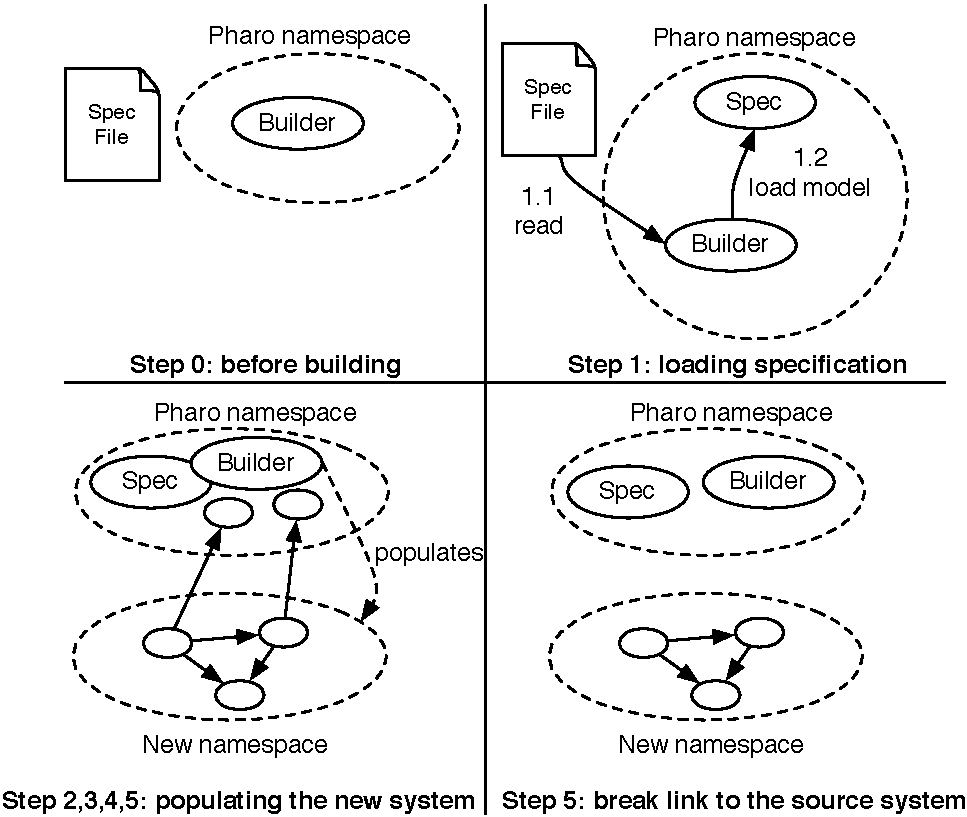
\includegraphics[width=0.6\linewidth]{hazelnut_overview}
\caption{Overview of Hazelnut process to bootstrap a reflective system\label{fig:hazelnut_overview}}
\end{center}
\end{figure}

% ===========================================================================
\subsection{Challenges of Bootstrapping a Reflective Object-Oriented System}
% ===========================================================================

\gp{new challenges}

\subsubsection{Isolation of the new language kernel} Bootstrapping a reflective language implies that both host and guest language kernels coexist in the same environment while the bootstrap process takes place. The \emph{guest} kernel has to be isolated from the host language kernel \ie it must have no references to objects from the host language kernel. There are two main reasons for this requirement:

\begin{description}
\item[Leaked references imply a dependency.] In the presence of leaked references, the host language cannot be discarded and thus, the guest language kernel cannot be used without the host.
\item[Cross-kernel interaction cause unexpected failures.] Leaked references may be used to perform unmediated method invocations from a language kernel to another. These \emph{cross language-kernel method invocations} without mediation provoke a failure in the method lookup mechanism. On method invocation, the VM looks up in the class hierarchy of the receiver a method with the same signature as the invocation~(\ie they have same \emph{identical} symbol as signature). Indeed, since each language kernel contains its own \ct{Symbol} class and symbol table, the method lookup mechanism fails.

%, since the language kernels are indeed different and the symbols to lookup in method dictionaries are not identical. Also, VM primitives do fail if they receive as argument an instance of a class from a different kernel, since they expect instances from the same language kernel.

\end{description}

\subsubsection{Tackle unicity hypothesis}
The infrastructural elements such as the VM or the compiler are built under the assumption that only one language kernel exists at runtime.
In the Pharo language the bytecodes and primitive invocations rely on the existence of only one copy of some special objects~(\eg \ct{nil}, \ct{true} or \ct{false}, and also objects with special formats such as strings, arrays, or methods). The virtual machine recognizes the special objects from the host language, and misbehaves with the ones from the guest language \eg sending the \ct{isNil} message to the \ct{nil} object from the host may result into \ct{true}, while sending the same message to the \ct{nil} instance from the guest may result into \ct{false}. This happens because the virtual machine assumes the existence of a single \ct{nil} object, the one from the host language~(cf. Figure \ref{fig:unicity_hipothesis}).

\begin{figure}[ht]
\center
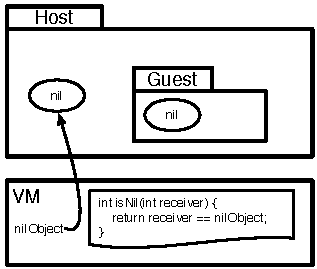
\includegraphics[width=.8\linewidth]{unicity_hipothesis}
\caption{\textbf{Example of the unicity hipothesis problem.} The Virtual Machine recognizes only the \ct{nil} object from the host language kernel as such. \label{fig:unicity_hipothesis}}
\end{figure}


\subsubsection{Avoid Logic duplications} During the bootstrap, the builder contains code to honor the invariants of those objects it creates inside the guest language kernel. These invariants are also present in the guest language specification. However, since the guest language kernel cannot execute its own code during the bootstrap process~(and thus, it cannot enforce its own invariants), this poses a logic duplication between the builder and the specification. To illustrate this problem with an example, consider the method \ct{Dictionary>>initialize:} used to initialize a \ct{Dictionary} instance, in Figure~\ref{code:logic_dup}:

\begin{figure}[ht]
\begin{code}
Dictionary>>initialize: n
    "Initialize array to an array size of n"
    array := Array new: n.
    tally := 0
\end{code}
\caption{\textbf{Code of the method \ct{Dictionary>>initialize}.}\label{code:logic_dup}}
\end{figure}

In order to respect the invariants of Dictionary initialization, the builder should execute some code as the one in Figure~\ref{code:logic_dup2}. This piece of code presents a logic duplication that cannot be easily eliminated. Note that this code, while written in Smalltalk syntax, would have the same form and problems if written in another language such as C.

\begin{figure}[ht]
\begin{code}
Builder>>createDictionaryWith: n
    "Initialize a dictionary in the language kernel"
    | dictionary internalArray |
    dictionary := self instantiate: 'Dictionary'.
    internalArray := self instantiate: 'Array' withSize: n.
    dictionary setInstanceVariable: 'array' with: internalArray.
    dictionary setInstanceVariable: 'tally' with: 0.
    ^ dictionary
\end{code}
\caption{\textbf{Code of the Builder implementing the same logic as in \ct{Dictionary>>initialize}.}\label{code:logic_dup2}}
\end{figure}

Additionally, the methods installed in the guest kernel must also honor the same invariants. This introduces a redundancy in the system: the code to manipulate the guest language in its early stages is duplicated with the code that will be installed in the final bootstrapped language, so the invariants of the guest language are always honored.

\gp{old challenges}

Meta-circularities make the process of building a new reflective system more complex than building a system without them. 
The building process should solve these meta-circularities and provide a working system.
Once solved, we say the meta-circularities are \emph{closed}.
Meta-circularities in a reflective system such can be illustrated with several examples:

\begin{description}
\item \emph{Reflective core are expressed in themselves.} The core of many reflective and dynamic languages such as 
Ruby, Smalltalk and even Java are self-referencing. For example, the \ct{Metaclass} class is an instance of the \ct{Metaclass} metaclass and vice versa, as shown in \autoref{fig:smalltalk_metacircularity}.
This leads to a recursive dilemma: how can each of these two entities be initially built without its defining pair.
Due to its importance in the system structure this meta-circularity should be mandatory solved during the first steps of the bootstrap. We call this, the \emph{basic structural meta-circularity} of the system.

\item \emph{Finding the order of construction is complex.} A class must receive the \ct{new} message to create a new object.
A method with the same selector is looked up in the class' metaclass hierarchy.
Since methods are objects, they have to be instantiated also.
The meta-circularity resides in the fact a first \ct{new} method should exist to define all methods.
\end{description}

Such self-references are also present in other languages with reflective capabilities: \eg in Java the ClassLoader is a class itself;
Ruby presents an object-model very similar to Smalltalk extended with mixins.

\begin{figure}[!ht]
\begin{center}
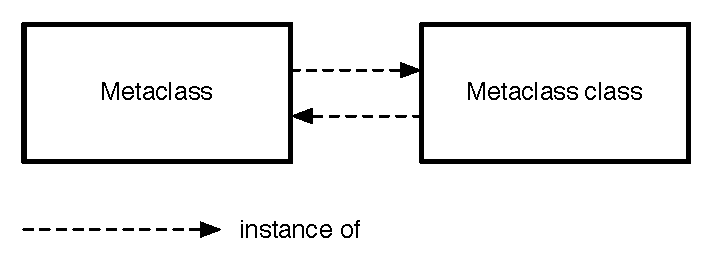
\includegraphics[width=0.40\linewidth]{smalltalk_metacircularity}
\caption{Smalltalk Metaclass circularity.\label{fig:smalltalk_metacircularity}}
\end{center}
\end{figure}

To solve these issues we proposed in a previous article the \emph{bootstrap of object-oriented reflective language kernels}~\cite{Poli13b}. By bootstrapping, the initialization of the language kernel is extracted from the VM and written in the same language it defines~(cf. Section \ref{sec:background}). Thus, the low level code is transformed in high level code, the language definition is decoupled from the VM initialization, and all its code is put together in one place. This solution has been shown to be effective but exposed some new challenges~(cf. Section \ref{sec:challenges}):
\begin{description}

\item[Isolation of the new language kernel.] The bootstrapped language kernel~(the \emph{guest} kernel) should be isolated from the language kernel executing the bootstrap process~(the \emph{host} kernel). The object graph of the guest kernel must fulfill the transitive closure property \ie have no references to objects of the host language. %Additionally, the tools residing in the bootstrapping language are not aware of the language that is being bootstrapped. Thus, they are not prepared to handle both languages at the same time and isolate each from the other.

\item[Tackle unicity hypothesis.] The infrastructural elements such as the VM or the compiler are built under the assumption that only one language kernel exists at runtime. Bootstrapping introduces a new language kernel on this infrastructure and breaks this assumption.

\item[Avoid Logic duplications.] Still some logic used to manipulate the object graph of the guest kernel during construction is duplicated with the code that will be installed inside the bootstrapped language kernel.

\end{description}

% ===========================================================================
\subsection{Object Spaces for Bootstrapping}
% ===========================================================================


We sketched the concept of object spaces in previous work~\cite{Poli13a}. We implemented with this purpose Oz\footnote{Not related to the Oz programming language. The name Oz for Pharo is inspired on the metaphor of multiple world manipulation.}, an extension of the Pharo programming implementing object spaces. An object space in Oz is composed by two main elements: the object runtime system it encapsulates and a \emph{membrane} of proxy objects controlling the interaction between the inner and outer runtime systems. The main purpose of these proxy objects is to hide the internal representation of the objects inside the object space. We consider these proxy objects mainly as mirrors~\cite{Brac04b}, as they expose only reflective behavior on the objects they represent \eg a mirror on a \ct{User} object cannot be manipulated in terms of its name or password, but only in terms of its instance variables and class.

When bootstrapping, the guest language kernel is hosted inside an object space. The builder manipulates and introspects the guest language kernel through this object space. The bootstrap process uses Oz through the following API to interact with its guest language kernel. Note that all operations will return a mirror instead of a reference to the corresponding object. The object space and its mirrors mediate all interaction with the objects inside the guest runtime system to ensure isolation~(Section \ref{sec:mirrors}):

\begin{description}
\item[Accessing well known objects.] Well known objects such as \ct{nil}, \ct{true} and \ct{false} can be get and set from an object space. The bootstrap process uses it during the well known instances initialization step. Once an object space is configured with such objects, it can execute code using them and overcome the \textbf{unicity hypothesis}.
\begin{code}
mirror getNil();
mirror getTrue();
mirror getFalse();

void setNil(mirror aNilObject);
void setTrue(mirror aTrueObject);
void setFalse(mirror aFalseObject);
\end{code}

\item[Object allocation.] Object allocation operations provide support for the initialization of the guest language kernel. In particular, \ct{allocateObjectOfSize()} is the unsafe operation used to instantiate the first objects when there are no classes available.
\begin{code}
mirror allocateObjectOfSize(int size);
mirror allocateObjectOfClass(mirror aClass);
mirror compile(String sourceCode, mirror aClass);
\end{code}

\item[Runtime system manipulation.] To initialize the classes in the guest language kernel, Oz provides with operations to install classes and obtain the list of classes installed.
\begin{code}
void installClass(mirror aClass);
List<mirror> getClasses();
\end{code}

\item[Code execution.] Oz provides with operations to manipulate the processes/threads of the guest language kernel. In particular, the \ct{runForTime()} operation will execute the guest language kernel with whichever processes it has installed, directly on the VM.
\begin{code}
List<mirror> getProcesses();
mirror createProcessDoing(String expression);
void runForTime(int milliseconds);
\end{code}
%\caption{\textbf{Code of the Builder implementing the same logic as in \ct{Dictionary>>initialize}.}\label{code:logic_dup2}}
%\end{figure}
\end{description}

\subsubsection{Ensuring Isolation through Mirrors}\label{sec:mirrors}

Oz provides access to the objects inside its inner runtime system through proxy objects. We consider these proxy objects as mirrors~\cite{Brac04b} as they provide only reflective operations on the objects they represent. These mirrors conform a \emph{membrane} that mediates the interaction between guest and host language kernels to keep them \textbf{isolated} from each other \ie object references from the guest language kernel do not leak into the host language kernel and vice-versa. To ensure isolation, mirrors provide the following API to interact with the objects they wrap:

\begin{description}
\item[Class access.] Method installation and object manipulation is achieved by class access operations. In particular, the \ct{setClass()} operation is used in the first steps of the bootstrap process to close the main circularities and set the class of the \ct{nil} object.
\begin{code}
mirror getClass().
void setClass(mirror aClass).
\end{code}

\item[Internal state access.] Every object initialization of the bootstrap process is achieved by altering their internal state. Mirrors provide a low level API to get and set the fields of an object.
\begin{code}
mirror getInstanceVariable(String variableName).
void setInstanceVariable(String variableName, mirror anObject).
\end{code}
\end{description}

Note from the signatures presented that all mirror operations will return a mirror in exchange, and so, interaction with other objects inside the object space is mediated by Oz. Mirrors could give and revoke permissions on the wrapped object and enforce invariants to keep the model consistent~\cite{Teru13a}.
Oz provides also specific kinds of mirrors with high level APIs to manipulate objects with a specific format and/or behavior such as classes, methods, activation records or processes. We do not cover high level mirrors in this paper because they are not relevant to the bootstrap process.

%An object space uses a cross compiler to generate methods for the guest language. %We based our cross compiler in the Opal compiler toolchain\cite{Bera13a}. 
%The cross compiler receives as input the source code to compile and a \ct{binding-resolver} object that defines how names will be resolved during compilation. The output of the cross compiler is both the bytecode for the guest object space and a list of literals that belong to the method and will be afterwards translated into their guest representation. The literal objects resolved during compilation are classified in two different categories:
%
%\begin{description}
%\item[Immediate Literal objects.]  These literal objects are translated from the host language to the guest language using the literal translation mechanism showed in Figure \ref{fig:cross_compiling}.
%\item[Name bindings.] Those objects that are accessed though a name, such as classes or class variables. These literals are resolved during compilation as symbolic references \eg if a method contains a reference to the class \ct{String}, after compilation, the list of literals will contain a \ct{GlobalBinding} object with the name of the referenced class~(\ct{'String'} in this case). In our implementation, we consider three main binding objects: \ct{GlobalBinding}, \ct{ClassVariableBinding} and \ct{UndefinedBinding}, which is used when the name could not be resolved.
%\end{description} 
%
%After compilation, the creation of a method takes place inside the guest language. The bytecodes are installed in this new method, and the literals are resolved inside the guest language. Figure \ref{fig:cross_compiling} shows the relationship between the source code, the binding objects and the final translated method.

%\begin{figure*}[ht]
%\begin{center}
%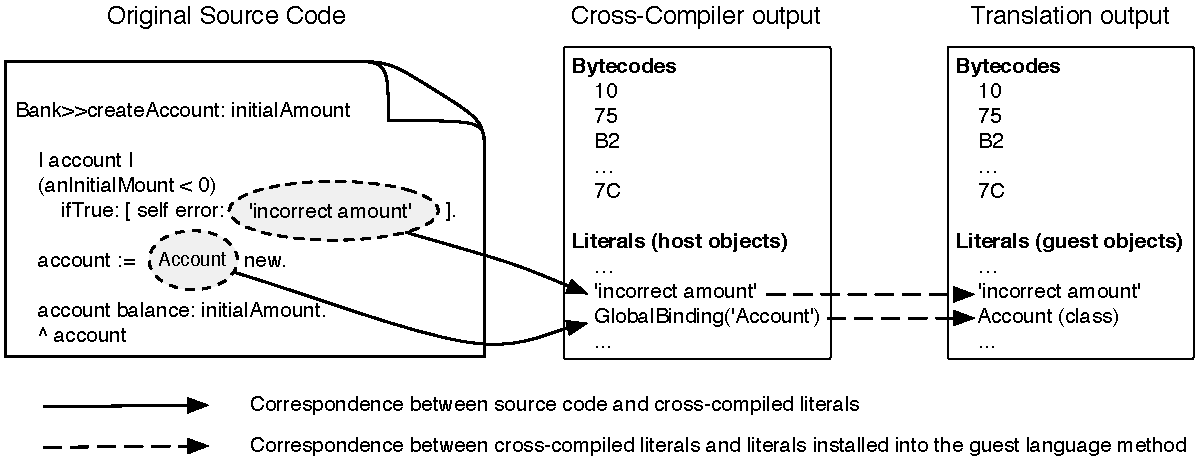
\includegraphics[width=.70\linewidth]{cross-compiling}
%\caption{\textbf{Mapping of literals from source code to their representation inside the guest language.} The cross compiler takes the original source code and outputs a list of bytecode and literals objects from the host language. Literal objects such as strings are resolved as normal string objects while class references are resolved as \ct{GlobalBinding} objects. Afterwards, the translation step transforms the host literal string to a guest literal string and the global binding is resolved into a reference to the class inside the guest language. \label{fig:cross_compiling}}
%\end{center}
%\end{figure*}


\subsubsection{Tackling Duplications with AST Interpretation}\label{sec:ast_interpreter}

To avoid logic and code duplications between the builder and the language kernel specification, we decided to use the kernel specification for both an input to compile the methods in the guest language kernel and to manipulate it. We use an AST interpreter to execute the code from the kernel specification inside the guest object space. Figure~\ref{code:logic_dup3} illustrates how the method in Figure~\ref{code:logic_dup2} can be rewritten to avoid the duplication with the original \ct{Dictionary} method from Figure~\ref{code:logic_dup}. Indeed the code in the example is simplified: since we would like to support the rename of class and method names, those names should not be hardcoded in the real code.

\begin{figure}[ht]
\begin{code}
Builder>>createDictionaryWith: n
    "Initialize a dictionary in the language kernel"
    ^ self astInterpreter
            execute: 'Dictionary new: size'
            binding: { 'size' -> n }.
\end{code}
\caption{\textbf{New code of the Builder using the same logic as in \ct{Dictionary>>initialize} without repetition.}\label{code:logic_dup3}}
\end{figure}

The AST interpreter provides with the following good properties to the bootstrap process:

\begin{description}

\item[Allow execution in non-yet causally connected systems.] The AST interpreter allows the execution of code inside the object space when classes have no methods installed. To do that the AST interpreter overrides the method lookup mechanism executing the code defined in the guest language specification. Internally, it uses a map that associates the classes inside an object space with their representation in the language specification to bootstrap.

\item[Avoid code duplication.] The AST interpreter uses the source code found in the new language specification to manipulate the guest language and compile methods in the guest language. Since the logic comes from a single source~(the language specification) there is \textbf{no code or logic duplication}. Thus, the only one point for extension or modification of the bootstrapped system is its specification.

\item[Provide hooks for primitive methods.] The AST interpreter allows one to control the execution at every step of it and provides hooks to intercept and change primitive methods. This way, the AST interpreter \textbf{overcomes the unicity hypothesis} exposed in Section \ref{sec:challenges}. 

\end{description}

The AST interpreter has two main points of interaction with Oz: access the well known objects needed for execution~(\ie \ct{nil}, \ct{true} and \ct{false}) and provide object fields' access~(\ie get a field of an object when it is accessed, and set a field of an object when it is assigned). Figure~\ref{fig:ast_interaction} shows the interaction between the AST interpreter and an object space when executing the first statement of the \ct{Dictionary>>initialize} method shown in Figure~\ref{code:logic_dup}. The object space is accessed to instantiate the \ct{Array} class, returning a mirror on it. Then, the mirror on the dictionary is in charge of assigning the array in the corresponding instance variable. The mirror dictionary unwraps the array before assignment to avoid introducing a mirror reference inside the guest language kernel.

\begin{figure*}[ht]
\center
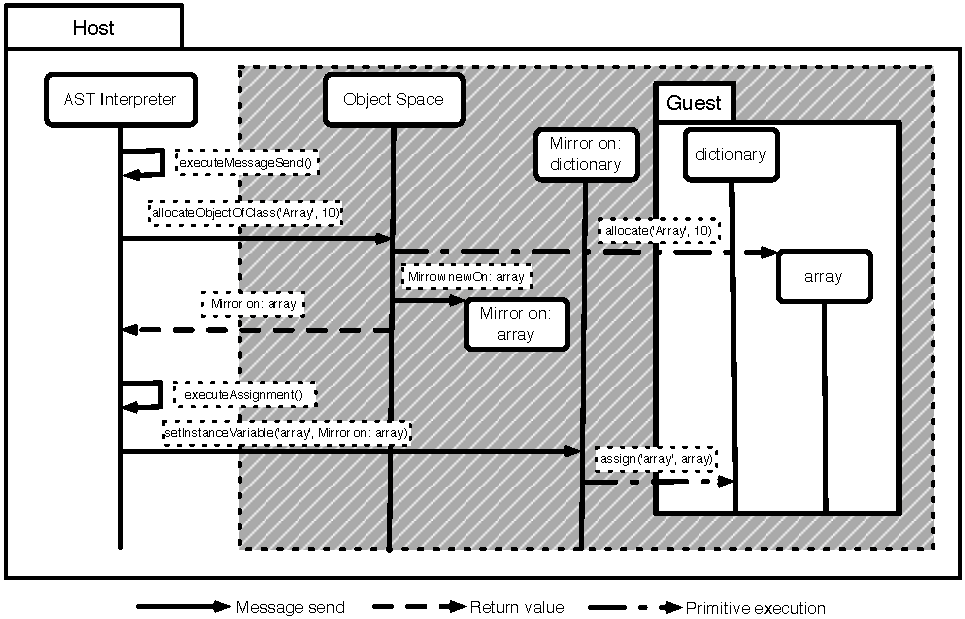
\includegraphics[width=1\linewidth]{AST_interaction}
\caption{\textbf{Illustrating the AST interpreter interaction with an object space and mirrors.} \label{fig:ast_interaction}}
\end{figure*}



% ===========================================================================
\section{Tailoring}
% ===========================================================================


% ===========================================================================
\subsection{Evolution by Tailoring} \label{sec:example_intro}
% ===========================================================================

Unused code units represent serious drawbacks in constrained devices. 
First, unused code units may forbid the deployment into a constrained resource device.
It may also interfere with the deployment and usage of other applications, because of large memory footprints in both secondary~(disk storage) and primary~(RAM) memory~\cite{Mart12a} or the presence of slow networks in the case of rich web applications.
Second, some deployment targets may have an infrastructure designed in such a manner that forbids the deployment of large applications. For example, the Android's Dalvik VM restricts an application to deploy only 65536 methods.

% ===========================================================================
\subsection{Reducing an Application's Memory Footprint, a Motivating Example} \label{sec:example_intro}
% ===========================================================================

To clearly show the problem, consider the application using a logging library in Figure~\ref{fig:example_dead_code}.
An interface is present in the diagram to show polymorphism between two classes that do not share a class inheritance hierarchy. 
However, some languages, such as the dynamically typed ones, may not need to represent it in the source code.

\begin{figure}[ht]
\begin{center}
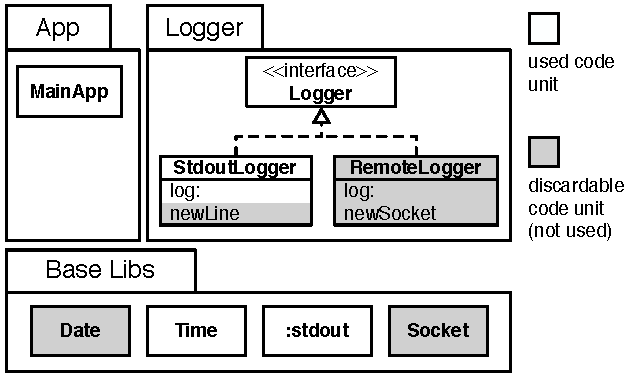
\includegraphics[width=.9\linewidth]{example_dead_code}
\caption{\small\textbf{Example of unused code units.} In gray, the unused code units that can safely be removed.\label{fig:example_dead_code}}
\end{center}
\end{figure}

Figure~\ref{fig:code_example1} shows the code of this application, written in the Pharo Smalltalk language. This application contains a \ct{MainApp} class with a \ct{start} method, which is the entry point of our application. The \ct{start} method creates an instance of \ct{Stdout\-Logger} and logs the application's start and end. In turn, the \ct{StdoutLogger} uses the \ct{stdout} global instance to log in the standard output the current time and the message. To print the time, the \ct{StdoutLogger} makes use of the \ct{Time} class from the base libraries of the language. Note that for the sake of clarity, we didn't include in the example all base libraries, though, in modern programming languages they represent a large codebase with several features going from networking to multithreading. For example, Java 8 SE contains 4240 classes\footnote{according to the javadoc API}, and the development edition of Pharo 2.0 contains 3342 classes and traits.

\begin{figure}[ht]
\begin{code}
MainApp>>start
    logger := StdoutLogger new.
    logger log: 'Application has started'.
    "do something"
    logger log: 'Application has finished'.

!\unusedcode{StdoutLogger>>newLine}!
!\unusedcode{~~~stdout newLine.}!

StdoutLogger>>log: aMessage
    stdout nextPutAll: Time now printString.
    stdout nextPutAll: aMessage.
    stdout newLine.
    
!\unusedcode{RemoteLogger>>log: aMessage}!
!\unusedcode{~~~| socket |}!
!\unusedcode{~~~socket := self newSocket.}!
!\unusedcode{~~~socket nextPutAll: Time now printString.}!
!\unusedcode{~~~socket nextPutAll: aMessage.}!
!\unusedcode{~~~socket newLine.}!

!\unusedcode{RemoteLogger>>newSocket}!
!\unusedcode{~~~"...."}!
!\unusedcode{~~~"creates an instance of socket given some configuration"}!
\end{code}

\caption{ \small\textbf{Code of the unused code units example.} In gray, methods not used by the application.\label{fig:code_example1}}
\end{figure}

In this example we can detect the following unused code units, shown in grey in Figure~\ref{fig:example_dead_code} and Figure~\ref{fig:code_example1}:
\begin{enumerate}
\item The logger library includes two logging classes~(\ct{Stdout\-Logger} and \ct{RemoteLogger}). Only the \ct{StdoutLogger} is used and thus, the \ct{RemoteLogger} class can be discarded.
\item Since the \ct{MainApp} class does not use the \ct{Socket} class nor the \ct{RemoteLogger} class~(the only user of the \ct{Socket} class), the \ct{Socket} class can be discarded.
\item No class in the application makes use of the \ct{Date} class. Then, this class can be safely removed.
\item The method \ct{newLine}~(lines 7-8 of Figure~\ref{fig:code_example1}) of the \ct{StdoutLogger} class is not used and can be also removed.
\item The \ct{StdoutLogger} class uses the \ct{Time} class to print the current time. Then, all code units that are not related to the \ct{Time now} resolution or printing~(\ie time arithmetic) could be considered as unused.
\end{enumerate}

We would like to generate a new version of this application not containing these unused code units while keeping the application's behavior. We call this technique \emph{Deployment Unit Tailoring} or \emph{Application Tailoring}.

% ===========================================================================
\subsection{A Tailoring Process for Reflective Languages}
% ===========================================================================

This paper describes \emph{Tornado}: an alternative solution to dead code elimination using a dynamic technique.
Tornado uses a run-fail-grow technique to identify during runtime those code units that are actually used in an application.
It consists in ``growing'' a seed into a deployable specialized version of an application. 
We feed this \emph{new} minimal version of the application (the \emph{seed}) with the missing code units needed to run.
The resulting deployable application only embeds the seed and used code.
By carefully choosing the seed, the user customizes the scope of the tailoring process making possible different levels of tailoring.
For example, a seed that includes all base libraries makes the tailoring process to only select used code in the application-specific part; whereas an empty seed makes the tailoring process to select used code in all parts: base libraries, application libraries and application-specific part.
% For example, if the seed includes the language base libraries, it ensures that the deployed application will have it all whereas an empty seed will result that only part of the base libs 
% Afterwards, deployment units are created from this shrank application to only contain the used code units.
% Using these compacted deployment units leverages the targeted device limitations. 
The dynamic nature of our solution allows its usage in dynamic languages, without type annotations. Our solution does not need to modify the original application thanks to its run-fail-grow approach.
It also successfully deals with applications that make use of programming language features such as reflection or open classes.


We propose Tornado, a run-fail-grow approach for tailoring. Tornado works by launching a \emph{nurtured} application that has only part of its required code units installed and a \emph{reference} application encompassing all the code units that resulted from the development process. When a failure is detected in the nurtured application, Tornado takes the missing code units from the reference application and install them into the nurtured application. Thus, the nurtured application grows progressively as failures are found.
Once finished, the nurtured application is ready to be deployed on target devices. Figure~\ref{fig:runfail} depicts the basics of our run-fail-grow approach.

%, in contrast with a trace-copy approach. Our run-fail approach avoids changing or manipulating the reference application, remaining unchanged from its original version.

\begin{figure}[ht]
\begin{center}
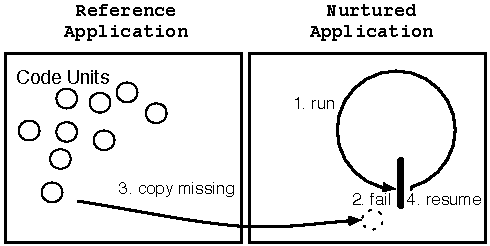
\includegraphics[width=.9\linewidth]{runfail}
\caption{\small \textbf{Application tailoring with a run-fail-grow approach.} We run the nurtured application~(1) and detects the missing units on failure~(2). At each failure, missing code units are installed from the reference application~(3) and the execution is resumed (just before the failure)~(4) until the process finishes. \label{fig:runfail}}
\end{center}
\end{figure}

% containing only \emph{application's entry points} (code units used to launch the application) 

Tornado starts by launching the reference application to create initial objects and perform startup computations. The reference application is then paused so its state do not change during the tailoring process. Pausing consists in suspending all processes and threads from the application.

Initially, the nurtured application is initialized with only a \emph{seed} embedding code units that developers want to ensure into the deployed application.
When the nurtured application starts from a seed that contains the language base libraries, the tailoring will only affect the application specific code units and third-party libraries.
When it starts from an empty seed, it will also tailor base libraries.

Following, it installs one or more \emph{application's entry points}.
An application's entry point consists in one or more statements that perform some initial computations of the application (\eg a \emph{main()} method in Java, or the initial method of a thread). 
The execution of an entry point will result into sending messages to some objects.
Required code units will then be cloned on demand from the reference application into the nurtured one.
Duplication is performed lazily.
For example, when duplicating a class, the content of its fields is not duplicated with it, but deferred until it is actually needed.
Also, methods are not duplicated until they are invoked.
The process repeats until the user ends it explicitly. Ideally, the nurtured application reaches a stable point where it needs no more code units.
The nurtured application is then ready for deployment.

% ===========================================================================
\subsection{Challenges of Application Tailoring} \label{sec:challenges}
% ===========================================================================

A lot of work exists on the tailoring of statically-typed applications~\cite{ShortCour10a,ShortRays02a,ShortTip03a,ShortPopa04a,ShortTeod01a}, where the type annotations aid in the resolution of which piece of code will be used during runtime. 
However, static analysis is not an option in the context of dynamically-typed languages or in the presence of meta-programming and reflection.\gp{should get a good cite for this last sentence}
%~\cite{Mart12a}
In this context of dynamically typed and object-oriented programs that may use reflection, we identify the following main challenges for detecting unused code units:

\begin{description}

\item[Dynamic typing.] Dynamic languages cannot benefit from static analysis due to the absence of type annotations. Those techniques used to detect used code units, such as call-graph analysis, need the support of more dynamic techniques such as tracking runtime information, following the application's execution flow, or performing symbolic execution.

\item[Polymorphism and inheritance.] Polymorphism in object-oriented languages allows a code unit to treat objects of different concrete types in the same way as soon as they share a common interface. Inheritance plays a similar role: any class can extend another class and provide different behavior while sharing the same API.
As a consequence, both polymorphism and inheritance make the behavior of a program more difficult to predict by just analyzing its code units~\cite{ShortTaen89a}.

\item[Base libraries are often VM managed.] In most of the modern object-oriented languages, base language libraries such as Java's bootstrap class loaders or native methods are loaded and initialized by the Virtual Machine~(VM) or some low-level component. Since most applications do not use all standard libraries even if they are initialized, these often big code bases are potentially candidates for removal. However, this raises a challenge since it often requires VM modifications.

\item[Application runtime configuration.] Modern applications often contain libraries and frameworks besides their proper code. 
To make these different code units fit together, applications rely on heavy configurations. 
These configurations are usually present in configuration files looked up dynamically by the application. 
Based on these configurations, the dependency injection pattern is usually used to dynamically set up the application. 
This recurrent and standard process for configuring applications implies that static analysis will be inefficient to detect used code units without library-specific knowledge.
 % The configuration code unit adds another dynamic element to the application, making its behavior more complex to predict with static approaches.

%\item[Application configuration granularity.] An application's configuration is not often granular. Libraries and frameworks may initialize during their startup lots of objects that are not used during the application's life cycle. These configuration objects may remain in static/class fields cached until the application is stopped, impacting in the memory footprint \gp{this is a problem, not a challenge. The challenge is to be able to detect unused objects in addition to methods}.

\item[Reflection.] Reflection makes static analysis inoperative by allowing an application to execute unanticipated pieces of code. 
Any \ct{String} resulting from a program execution or program configuration can denote a message send\footnote{We refer method invocations as message sends because they represent better from our understanding the dynamic property of the invocation.}, the name of a class to be instantiated, or even a script to be executed. Reflection is indeed important to cover, since it is a broadly used tool in industrial applications with object relational mappers such as Hibernate or Glorp and web frameworks such as Ruby On Rails, Struts or Seaside.

\end{description}


%============================================================================
\subsection{Object Spaces support for Tailoring}
%============================================================================

\gp{make explicit that Tornado requires a special infrastructure to run => it needs 'only' during the process to access classes, install methods, stop execution. It also needs a way to extract the code units that were installed for deploy.}

Tornado is based on an architecture that allows complex manipulation of both the nurtured and the reference applications. Examples of such complex manipulations are \eg Tornado must be notified when a failure occurs in the nurtured application because some code unit is missing, it should be able to start/pause/stop its execution at safe points, install missing code units such as classes and methods, and query runtime information from both the reference and nurtured applications. Our approach performs those tasks through the manipulation of the \emph{object runtime systems} of the applications. An object runtime system is a runtime system of an object-oriented application \eg a running Java virtual machine executing a Java program, and thus, containing the objects and classes of the application. We identify the following components as part of Tornado's architecture~(cf. Figure~\ref{fig:tornado_code units}):

\begin{description}
\item[Object runtime manipulation interface.] An object runtime manipulation interface allows one to act over an object runtime system by controlling its runtime execution~(\eg starting, pausing and restarting it, and installing new threads/processes) and perform introspection and intercession~(\eg installing classes and methods, retrieve the loaded classes) on it. A well known example of such an interface is the JVM TI~(JVM tool interface)~\cite{JVMTI}.
We use this module to pause the reference application, suspend the execution of the nurtured application when a failure is detected, get the methods to install from the reference application, and install the necessary methods and classes into the nurtured application.

\item[Advanced intercession module.] An advanced intercession module allows advanced reflective capabilities such as modifying an object's behavior during runtime. Tornado uses this module to capture message sends and so to be notified when it finds missing code units. JRebel~\cite{Jreb12a}, Reflectivity~\cite{Denk08a} or Bifrost~\cite{Res12} are examples of such intercession libraries.

\end{description}

\begin{figure}[ht]
\begin{center}
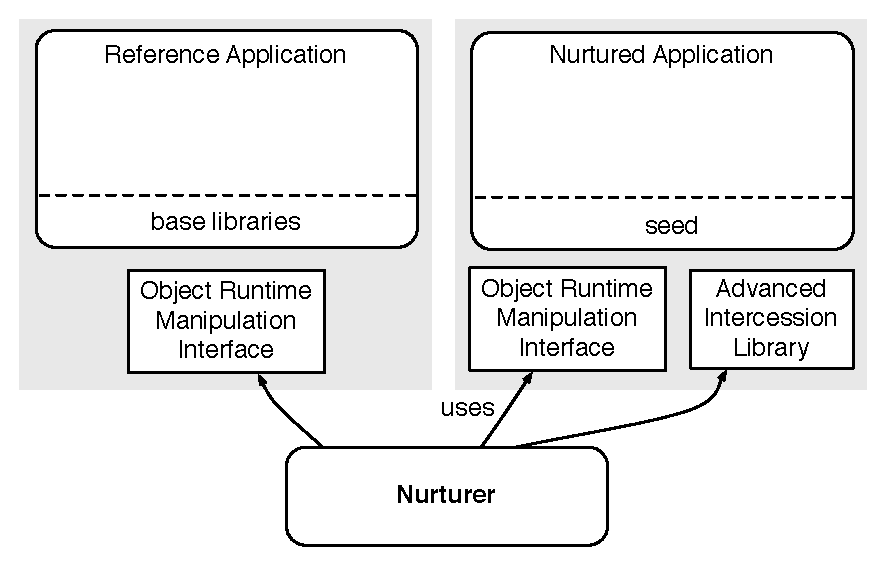
\includegraphics[width=0.95\linewidth]{tornado_components2}
\caption{\small\textbf{Tornado's architecture overview.}\label{fig:tornado_code units}}
\end{center}
\end{figure}


\subsection{The object runtime manipulation interface: Oz object spaces}

Tornado monitors the execution of the nurtured application and manipulates it during runtime as explained in Section~\ref{sec:infrastructure}.
We built Tornado using our Oz\footnote{Not related to the Oz programming language. The name Oz for Pharo is inspired on the metaphor of multiple world manipulation.} object spaces~\cite{Poli13a} solution as the \emph{object runtime manipulation interface}. Oz is an extension of the Pharo programming language implementing \emph{protection domains} so called \emph{object spaces}. Oz presents a first class representation of an object space providing a high level API to manipulate those protection domains.

In our Tornado implementation, the reference and nurtured applications are contained each in a different object space. Tornado places traps inside the nurtured object space and starts its execution. This execution is performed directly on a Pharo Virtual Machine, and thus, there is no speed overhead as soon as traps are not involved. Whenever the nurtured object space's execution founds a trap, it pauses and returns the control to Tornado. Tornado inspects the classes and methods in the reference object space through mirrors~\cite{ShortBrac04b} and installs the needed code units from the reference object space on demand, either by creating new objects or compiling new methods. Then, it restarts the nurtured object space's execution from the message send that activated the trap.

\subsection{Related Work}

 \begin{table*}[ht]
 \small
 	\centering
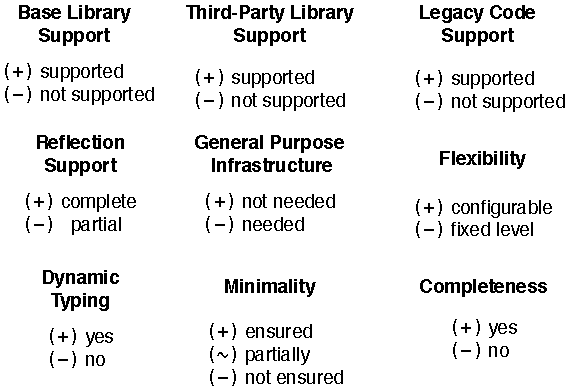
\includegraphics[width=\linewidth]{criteria_overview}
 	\begin{tabular}{|ccccc>{\columncolor[gray]{0.8}}c|}
	
\hline
 			& \textbf{Dedicated}
 			& \textbf{Static}
			& \textbf{Hybrid}
 			& \textbf{Dynamic}
 			& \textbf{Tornado} \\
 			& \textbf{SDKs}
 			& \textbf{Analysis}
			& \textbf{Analysis}
 			& \textbf{Analysis}
 			& \\
%  \cmidrule(r){2-6}
% \midrule

		Base Library&&&&&\\Support
 			& + & + & + & + & +\\
		\hline
		Third-Party&&&&&\\ Library Support
 			& - & + & + & + & +\\
		\hline
		Legacy Code&&&&&\\ Support
 			& - & + & + & + & + \\
		\hline
		Reflection&&&&&\\ Support
 			& + & - & - & + & + \\
		\hline
		Special&&&&&\\ Infrastructure& - & + & - & - & + \\for Running
 			&&&&&\\
		\hline
		Flexibility
 			& - & - & - & - & +  \\
 	 \hline
 	\end{tabular}
 	\caption{Evaluation criteria applied to related work on deployment code unit tailoring techniques}
 	\label{tb:comparison}
 \end{table*}
 
The reduction of the deployment footprint of object-oriented applications has been subject of interest both in industry and research since many years. In such regard, we identified four different families of solutions for dead code elimination: dedicated SDKs~(cf. section \ref{section:static_selection_rw}), static analyses~(cf. section \ref{section:static_rw}), dynamic analyses~(cf. section \ref{section:dynamic_rw}) and hybrid analyses~(cf. section \ref{section:hybrid_rw}). Table~\ref{tb:comparison} presents a comparison of these techniques, given the criteria defined in section~\ref{sec:criteria}.

\subsection{Dedicated SDKs}%Pre-conceived specialized application-independent platforms}
\label{section:static_selection_rw}

Dedicated SDKs are SDKs containing frameworks and/or libraries prepared to run under specific circumstances. For example, Java Micro Edition~(J2ME)~\cite{JavaME} as the dedicated version of the Java SDK, or Cocoa Touch as the one of Cocoa. These specialized SDKs are reduced platforms to run applications inside mobile and constrained devices. These platforms provide a reduced and fixed set of base libraries defined a priori and in a not customizable way. Applications have to be written especially for them, and thus legacy code and third-party libraries not written especially for it are not compatible. Reflection is available since the statically tailored base libraries are built in a not automatic fashion, and the application code is not tailored.

\subsection{Static Analysis-Based Techniques}\label{section:static_rw}

Static analysis approaches for dead code elimination make use of the static information of a program to select the minimal subset of used elements. The bibliography describes four different algorithms to achieve this goal: unique name, class hierarchy analysis~(CHA), rapid type analysis~(RTA) and reachable members analysis~(RMA) \cite{Baco96a, Titz06a}. These techniques share a common approach, selecting an entry point method of an application and following from it the execution flow using the available static information \ie type annotations, and class and method names, building a call-graph~\cite{ShortGrov97a}.

These techniques have been studied and applied in many environments and languages. Rayside et al.~\cite{ShortRays02a}, Jax~\cite{ShortTip03a} and the ExoVM System~\cite{Titz06a} propose application extraction tools using these techniques for Java applications. Sallenave et al.~\cite{Sall10a} apply RTA to produce smaller .NET assemblies for embedded systems. Bournoutian et al.~\cite{Bour14a} use CHA to optimize on-device Objective-C applications.

In summary, these approaches are based on the static types found either in the source code or byte code. Thus, they are not applicable efficiently in dynamic languages with no static type information. These solutions are valuable as they allow one to tailor base and third-party libraries, and legacy code. Their tailoring approach generates new deployment units that can run on the standard runtime infrastructure. The main drawback of this approach appears in the presence of reflection and configuration files, which will only work with a subset of reflective invocations through complementary analyses on the strings found in the source code. Also, existing solutions in this family lack the flexibility to declare and identify levels of tailoring, making it an "all or nothing".

\gp{Closed World Assumption kills you guys!}

\subsection{Dynamic Analysis-Based Techniques}\label{section:dynamic_rw}

Dynamic analysis techniques use exclusively runtime information~(\ie execution flow, alive objects, execution statistics) to perform dead code elimination. Amongst these, we identify two different approaches: \emph{load on demand} and \emph{code collection}. Load on demand approaches detect during runtime whenever a class or method needs to be installed and request it to a server application. Code collection approaches deploy the full application  and garbage collect unused code based on usage statistics. Related work in this family share a common characteristic: these techniques are used inside ubiquitous systems \ie systems meant to be always connected. Ubiquitous systems, as they are always connected, have a possibility to fallback and recover in the case of incompleteness. However, to focus here on the dead code elimination techniques, we will discuss the incompleteness recovery techniques in section \ref{section:completeness}.

JUCE~\cite{ShortPopa04a,ShortTeod01a} is a platform for ubiquitous devices supporting code load on demand and code collection. Its approach for building up an application is similar to Tornado's. First, it initializes a minimal running application and code is loaded, with a method granularity, from a server located in a different machine. Unused code is collected following usage statistics, and loaded back again on demand if needed.

OLIE~\cite{Gu03a} is an engine that intelligently partitions and offloads objects during runtime to minimize memory consumption. It is part of the adaptive infrastructure for distributed loading (AIDE). In OLIE, offloaded objects are indeed migrated to nearby remote devices. Migrated objects can be accesses later through proxies that perform remote invocations on them.

SlimVM~\cite{Kers09a, Wagn11a} is an ubiquitous system where all code resides on a remote server and is loaded only on demand on small devices. Some static analysis is performed only on the server to reduce the size of the transported code, by identifying most likely needed code. SlimVM changes the class format,  However, on the client side, every code load is done dynamically.

All solutions inside this category share one main property: they require to run the application inside a special infrastructure to apply their techniques \eg specialized VMs implementing remote lazy loading, code collection or special bytecode sets. The main challenge of these solutions resides on applying these techniques while minimizing their impact on performance during the runtime. Additionally, these solutions require their applications to run exclusively inside their infrastructure. Tornado works in the same way as these solutions: it uses a special infrastructure to run the desired application and select the used elements.  However, Tornado provides also with the ability to extract this application and run in \emph{offline} mode, using the non-modified infrastructure.

Regarding dynamic features such as reflection, this kind of solutions are the ones that can, potentially, handle it in the best way since they have in runtime all the information needed to resolve it. JUCE and OLIE, as Tornado, handle naturally reflection as they do not change the runtime representation (which programs make assumptions of, when they use metaprogramming). SlimVM on the other side, had to change the reflection support because they changed the object and class representation on their VM.

Regarding its applicability, SlimVM needs to recompile the whole application into its own format, while OLIE and JUCE, as Tornado, can tailor base and third party libraries without any modifications on it. Thus, the latter two can be applied to legacy code also for free. None of these solutions provide with the ability to select the level of tailoring always working on the full application. In contrast, Tornado uses Seeds to force a minimal subset of elements to be part of the application.


\subsection{Hybrid Analysis-Based Techniques}\label{section:hybrid_rw}

Hybrid analysis techniques mix static and dynamic~(\ie runtime) information to provide better results. The common approach of these is to start an application, such as Tornado does, and pause it after some minimal runtime information is available \ie call stacks are created, some classes are loaded and initialized, and some objects are instantiated. Then, it uses the built stack of alive objects to perform a static analysis, as described in section \ref{section:static_rw}, with concrete type information.

Java in The Small (JITS)~\cite{ShortCour10a} uses a hybrid approach to select the used parts of a program, and then loads them inside a binary image. A specialized VM loads the binary image at startup. JITS's approach tailors base and third-party libraries as well as application specific code. It does not require modifications on the existent application to tailor it, so a legacy application could theoretically be tailored with this approach. JITS does not offer the possibility to configure the tailoring level, since it was designed to be used only in embedded devices where no more than one application would be running. Regarding reflection, JITS presents the same drawbacks as the other static call graph analysis approaches since not all the runtime information about the reflective invocations can be deduced.

\section{Runtime Surgery?}

??

% ===========================================================================
\subsection{Evolving During Runtime}
%============================================================================

% ===========================================================================
\subsection{Performing Modifications on Runtime}
%============================================================================

% ===========================================================================
\subsection{Challenges}
%============================================================================

% ===========================================================================
\subsection{Object Spaces support for Runtime Modifications}
%============================================================================

% =============================================================================
\input{chapter-footer.tex}